\documentclass[11pt,a4paper,fontset=none]{ctexart}

\setCJKmainfont{WenQuanYi Micro Hei}[AutoFakeBold=2.5,AutoFakeSlant=0.15]
\setCJKsansfont{WenQuanYi Micro Hei}[AutoFakeBold=2.5]
\setCJKmonofont{WenQuanYi Micro Hei Mono}[AutoFakeBold=2.5]

\usepackage{geometry}
\geometry{margin=2.15cm,headheight=14pt}
\usepackage{amsmath,amssymb}
\usepackage{booktabs,longtable,array,pdflscape,ragged2e}
\usepackage{graphicx,placeins}
\usepackage{caption}
\usepackage[hidelinks]{hyperref}

\captionsetup{font=small,labelfont=bf,skip=6pt}
\setlength{\tabcolsep}{4.5pt}
\renewcommand{\arraystretch}{1.12}

\newcommand{\Dcf}{\ensuremath{\Delta_{\mathrm{cf}}}}
\newcommand{\meanmin}[2]{#1\,{\scriptsize(#2)}}

\title{十站点概念漂移的主驱动识别\\[0.35em]
\normalsize 2026\,年\,10\,月\,27\,日实验纪要}
\author{本机当日跑完的结果\\
\normalsize 数据与表来自 \texttt{cursor/10site-cd-primary-driver-a248}\\
\normalsize 提交 \texttt{a3545e6}，太平洋时间 2026-10-27 02:10}
\date{太平洋时间 2026\,年\,10\,月\,27\,日}

\begin{document}
\maketitle

\begin{abstract}
\noindent
今天在本仓库上跑完并落盘的实验，是一套十站点的概念漂移基准。协变量来自 ACS\,2018 加州 person 文件上的两个 WhyShift 任务：收入是否超过五万美元，以及是否享有公共医疗保险。十个站点共用同一份经验分布 \(P(X)\)。预烧四个批次之后，从第\,8\,个批次起，五个站点写入彼此不同的概念漂移，四个站点保持真实标签，一个站点把标签换成公平硬币。

主分数 \(\Dcf\) 是等样本量的 Brier 差，乘上本地模型相对抛硬币的技能，再在全样本和 \(X_1\) 的上下尾里取最大。在满强度、突然激活、线性规则作用于 \(X_1\) 中位数以上这一格上，\(\Dcf\) 把五个结构化漂移站点全部排在干净站点和噪声站点之前。两个任务、四个种子的配对一致率都是 \(1.000\)，最差种子也是 \(1.000\)。按 \(\Dcf\) 取出的前五个站点，就是这五个漂移站点。

协变量对照停在机会水平附近。边际标签总变差同样接近一半，因为结构化规则在被改写的行上对齐了基线正例率。噪声站点会抬高未加权的伪结果平方和、合并参考模型的 Brier 超额，以及联合 C2ST。技能门把这条假驱动拿掉。工作边界在弱改写和薄尾部：改写概率降到 \(0.4\)，或者线性规则只作用在工时的 \(0.9\) 分位以上，一致率落到 \(0.8\) 以下。
\end{abstract}

\tableofcontents

\section{当天跑完的实验}

全部计分都在 2026\,年\,10\,月\,27\,日上午完成，下面的钟点是太平洋时间。主结果写在分支 \texttt{cursor/\allowbreak 10site-cd-\allowbreak primary-driver-a248} 的提交 \texttt{a3545e6}（世界时 09:10，太平洋时间 02:10）。定稿表在 \texttt{experiments/\allowbreak primary\_driver\_\allowbreak 10site/results/}。本纪要里的数字是从这些 CSV 重新汇总的，三位小数与仓库里的 \texttt{RESULTS.md} 一致；不一致的地方按代码和 CSV 更正，并在第\,\ref{sec:reading} 节写明。

\begin{table}[ht]
\centering
\caption{当天的运行清单。带星号的行没有进入定稿 CSV。}
\label{tab:runs}
\small
\begin{tabular}{@{}lll>{\raggedright\arraybackslash}p{6.5cm}@{}}
\toprule
时间 & 运行 & 耗时 & 结果 \\
\midrule
01:53 & 合成烟雾，旧分数\(^{*}\) & 2.8\,秒 & 一致率 \(0.850\)。文件随后删除。 \\
01:53 & 收入，种子\,0，整窗 \(\Dcf\)\(^{*}\) & 20\,秒 & 漂移均值 \(0.110\)，干净 \(0.000\)，噪声 \(0.001\)。 \\
01:55 & 合成烟雾，区域最大\(^{*}\) & 2.0\,秒 & 一致率 \(1.000\)。漂移均值 \(0.108\)。 \\
01:55 & 收入，种子\,0，区域最大 & 25\,秒 & 漂移 \(0.288\)，干净 \(0.004\)，噪声 \(0.001\)。并入主套件。 \\
01:56 & \texttt{test\_dgp}\(^{*}\) & --- & 打印 \texttt{dgp invariants ok}。 \\
01:56 & 主套件，\texttt{--seeds 4} & 约\,8\,分钟 & 两个任务各四个全量重复，外加 \(q\in\{0.5,0.7\}\) 的敏感性格子。 \\
02:06 & 收入，薄尾与弱强度 & 128\,秒 & \(q\in\{0.8,0.9\}\)，三十六格，轻量打分器。 \\
02:08 & 报告与五张图 & --- & \texttt{RESULTS.md}、\texttt{summary.json}、五张 PNG。 \\
\bottomrule
\end{tabular}
\end{table}

定稿的 \texttt{site\_scores.csv} 有 770 行、25 个设计格。其中主格是两个任务、\(\alpha=1\)、突然激活、\(q=0.5\)、种子 \(0\)--\(3\)，带时间曲线、C2ST、概念组重要度和特征重要度。其余 23 格只在收入任务上、种子 \(0\)--\(2\)，用轻量随机森林，不计算 C2ST、概念组、特征重要度和时间曲线。\(\alpha=1\)、突然激活、\(q=0.5\) 这一行没有用轻量打分器重跑，敏感度表里的这一格就是主套件的四个全量种子。

同日还看过 ACS Mobility（\(80{,}329\times 21\)）和 ACS Employment（\(378{,}817\times 16\)）的形状，没有计分。TableShift、HELOC、Voting、ACIC\,2016 和 Taxi 没有跑。非线性规则的子组版本代码里有，这次没有用。

用户画布里另有一份当天上午写的「条件分布反事实」五层记录。那份记录的原始日志不在本仓库，附录\,\ref{app:cf} 只转写已经写进画布的判定，不把它算进上面这 770 行。

\section{设计}
\label{sec:design}

每个任务先丢掉非有限行。收入任务剩下 \(195{,}665\) 行、10 个官方协变量，正例率 \(0.411\)，标签是收入超过五万美元。\(X_1\) 是每周工时 WKHP，\(X_2\) 是学历 SCHL，\(X_3\) 是年龄 AGEP。公共医疗保险任务剩下 \(138{,}554\) 行、19 个官方协变量，正例率 \(0.369\)。\(X_1\) 是年龄，\(X_2\) 是学历，\(X_3\) 是个人收入 PINCP。

一次重复先在 \(16{,}000\) 行的分析样本上做缩尾标准化，再随机切成十个站点，每站 \(1{,}600\) 行。时间是合成的：\(16\) 个批次，每批 \(100\) 行。前四个批次所有站点都用真实基线标签。从 \(t^{\ast}=8\) 起：

\begin{itemize}
\item S0--S3 继续用基线标签。
\item S4--S6 只在 \(X_1\) 高于分析样本分位数的行上，把标签改成站点自己的线性半空间。三个系数是 \((1,0.35)\)、\((0.25,1)\)、\((-0.85,0.55)\)。方向取与基线标签更不一致的一侧，再把被改写行的正例率拉回基线正例率。
\item S7 在激活后的全部行上使用乘积 \(X_1 X_2\)。S8 使用 \(\sin(X_1)+X_3^{2}\)。两条非线性规则同样做正例率匹配。
\item S9 把激活后的标签换成 \(\mathrm{Bernoulli}(0.5)\)，故意不做正例率匹配。它破坏共识，不是主驱动。
\end{itemize}

\(\alpha\) 是一条已激活的行真正被改写的概率。突然激活在 \(t\ge 8\) 时权重为 \(1\)。渐进激活用四个批次把权重从 \(0\) 拉到 \(1\)，权重是 \(\min\{1,(t-8+1)/4\}\)。主格取 \(\alpha=1\)、突然激活、线性分位 \(q=0.5\)。

工时在 \(40\) 小时有一个尖峰。全样本上，\(0.5\) 和 \(0.7\) 分位都落在 \(40\)，严格高于该分位的比例同为 \(0.226\)。所以 \(q=0.5\) 和 \(q=0.7\) 选中的是同一批人。这两列都跑过，数值逐格相同；正文的敏感度表只留 \(q=0.5\)。\(0.8\) 分位是 \(45\) 小时，线性站点上被改写的比例大约 \(0.173\)；\(0.9\) 分位是 \(50\) 小时，大约 \(0.078\)。

\section{分数}

参考模型只用预烧窗口。每个站点在最近六个批次上做三折交叉拟合。主格的随机森林是 \(25\) 棵树、深度 \(8\)、叶节点最少 \(5\) 个样本、置换重复 \(3\) 次。轻量格是 \(20\) 棵树、深度 \(7\)、置换重复 \(2\) 次。

记 \(\mu_{\mathrm{ref}}^{(n)}\) 为把参考模型压到与本地样本等量后的预测，\(\mu_{\mathrm{loc}}\) 为本地交叉拟合预测。技能是
\[
\mathrm{skill}=\max\bigl\{2(\mathrm{AUC}_{\mathrm{loc}}-1/2),\,0\bigr\}.
\]
三个区域是全样本，以及预烧期 \(X_1\) 的上尾和它的补集。区域只用协变量。主分数取三个区域里技能门控 Brier 差的最大者：
\[
\Dcf
=
\max_{r}
\Bigl(
\mathrm{Brier}\bigl(\mu_{\mathrm{ref}}^{(n)},r\bigr)
-
\mathrm{Brier}\bigl(\mu_{\mathrm{loc}},r\bigr)
\Bigr)
\times
\mathrm{skill}.
\]
\(\texttt{delta\_cf\_global}\) 只保留全样本那一项，用来看子组漂移被未改写的行稀释之后还剩多少。

\(\tau^{2}\) 是同一对预测的均方差，对应伪结果分解里的概念项。不乘技能时，噪声站点也会很大。门控版本乘上同一个技能。等样本量 Brier 差本身不乘技能；合并参考模型用的是更大的参考样本，样本量差会留在分数里。

配对一致率是严格大于的比例。\(\mathrm{CD}>\mathrm{clean}\) 的分母是 \(5\times 4=20\) 对。设计目标是 \(\Dcf\) 的这一一致率高于 \(0.8\)。Pareto 分数是秩的相反数，所以一致率仍然是「漂移站点排在前面」的比例。主格的八次全量重复带有时间曲线，秩用三条轴：\(\Dcf\)、技能门控后的 \(\tau^{2}\)，以及
\[
\mathrm{time\_jump}
=
\max_{t\ge t^{\ast}}\Dcf(t)
-
\max_{t<t^{\ast}}\Dcf(t).
\]
敏感性格子没有曲线，秩只用前两条轴。仓库里的 \texttt{RESULTS.md} 只写了前两条，那一句对主格偏窄；本纪要按 \texttt{add\_pareto} 更正。

\section{主格：谁排在干净站点前面}
\label{sec:main}

表\,\ref{tab:concord-concept} 和表\,\ref{tab:concord-control} 是主格的平均一致率，括号里是四个种子里的最小值。概念分数这一组里，\(\Dcf\)、整窗 \(\Dcf\)、两种 \(\tau^{2}\)、等样本量 Brier 差和 Pareto 秩在两个任务上的五个对比都是 \(1.000\)。

\begin{landscape}
\begin{table}[p]
\centering
\caption{主格概念分数的配对一致率。单元格是四个种子的平均，括号内是最差种子。主格：\(\alpha=1\)，突然激活，\(q=0.5\)。}
\label{tab:concord-concept}
\footnotesize
\begin{tabular}{@{}llccccc@{}}
\toprule
任务 & 分数 & CD\(>\)clean & CD\(>\)noise & 线性\(>\)clean & 非线性\(>\)clean & CD\(>\)其余 \\
\midrule
收入 & \(\Dcf\) & \meanmin{1.000}{1.000} & \meanmin{1.000}{1.000} & \meanmin{1.000}{1.000} & \meanmin{1.000}{1.000} & \meanmin{1.000}{1.000} \\
收入 & 整窗 \(\Dcf\) & \meanmin{1.000}{1.000} & \meanmin{1.000}{1.000} & \meanmin{1.000}{1.000} & \meanmin{1.000}{1.000} & \meanmin{1.000}{1.000} \\
收入 & \(\tau^{2}\)，技能门控 & \meanmin{1.000}{1.000} & \meanmin{1.000}{1.000} & \meanmin{1.000}{1.000} & \meanmin{1.000}{1.000} & \meanmin{1.000}{1.000} \\
收入 & \(\tau^{2}\)，未加权 & \meanmin{1.000}{1.000} & \meanmin{1.000}{1.000} & \meanmin{1.000}{1.000} & \meanmin{1.000}{1.000} & \meanmin{1.000}{1.000} \\
收入 & 等量 Brier 差 & \meanmin{1.000}{1.000} & \meanmin{1.000}{1.000} & \meanmin{1.000}{1.000} & \meanmin{1.000}{1.000} & \meanmin{1.000}{1.000} \\
收入 & 合并参考 Brier 差 & \meanmin{1.000}{1.000} & \meanmin{0.400}{0.400} & \meanmin{1.000}{1.000} & \meanmin{1.000}{1.000} & \meanmin{0.880}{0.880} \\
收入 & Pareto 秩 & \meanmin{1.000}{1.000} & \meanmin{1.000}{1.000} & \meanmin{1.000}{1.000} & \meanmin{1.000}{1.000} & \meanmin{1.000}{1.000} \\
收入 & 本地技能 & \meanmin{0.938}{0.800} & \meanmin{1.000}{1.000} & \meanmin{1.000}{1.000} & \meanmin{0.844}{0.500} & \meanmin{0.950}{0.840} \\
\midrule
医保 & \(\Dcf\) & \meanmin{1.000}{1.000} & \meanmin{1.000}{1.000} & \meanmin{1.000}{1.000} & \meanmin{1.000}{1.000} & \meanmin{1.000}{1.000} \\
医保 & 整窗 \(\Dcf\) & \meanmin{1.000}{1.000} & \meanmin{1.000}{1.000} & \meanmin{1.000}{1.000} & \meanmin{1.000}{1.000} & \meanmin{1.000}{1.000} \\
医保 & \(\tau^{2}\)，技能门控 & \meanmin{1.000}{1.000} & \meanmin{1.000}{1.000} & \meanmin{1.000}{1.000} & \meanmin{1.000}{1.000} & \meanmin{1.000}{1.000} \\
医保 & \(\tau^{2}\)，未加权 & \meanmin{1.000}{1.000} & \meanmin{1.000}{1.000} & \meanmin{1.000}{1.000} & \meanmin{1.000}{1.000} & \meanmin{1.000}{1.000} \\
医保 & 等量 Brier 差 & \meanmin{1.000}{1.000} & \meanmin{1.000}{1.000} & \meanmin{1.000}{1.000} & \meanmin{1.000}{1.000} & \meanmin{1.000}{1.000} \\
医保 & 合并参考 Brier 差 & \meanmin{1.000}{1.000} & \meanmin{1.000}{1.000} & \meanmin{1.000}{1.000} & \meanmin{1.000}{1.000} & \meanmin{1.000}{1.000} \\
医保 & Pareto 秩 & \meanmin{1.000}{1.000} & \meanmin{1.000}{1.000} & \meanmin{1.000}{1.000} & \meanmin{1.000}{1.000} & \meanmin{1.000}{1.000} \\
医保 & 本地技能 & \meanmin{1.000}{1.000} & \meanmin{1.000}{1.000} & \meanmin{1.000}{1.000} & \meanmin{1.000}{1.000} & \meanmin{1.000}{1.000} \\
\bottomrule
\end{tabular}
\end{table}
\end{landscape}

\begin{landscape}
\begin{table}[p]
\centering
\caption{主格对照分数的配对一致率。括号内是最差种子。Domain AUC 和 MMD 只用协变量。标签总变差只用边际 \(Y\)。}
\label{tab:concord-control}
\footnotesize
\begin{tabular}{@{}llccccc@{}}
\toprule
任务 & 分数 & CD\(>\)clean & CD\(>\)noise & 线性\(>\)clean & 非线性\(>\)clean & CD\(>\)其余 \\
\midrule
收入 & 联合 C2ST & \meanmin{0.850}{0.800} & \meanmin{0.350}{0.200} & \meanmin{0.750}{0.667} & \meanmin{1.000}{1.000} & \meanmin{0.750}{0.680} \\
收入 & C2ST 缺口 & \meanmin{0.875}{0.700} & \meanmin{0.400}{0.400} & \meanmin{0.792}{0.500} & \meanmin{1.000}{1.000} & \meanmin{0.780}{0.640} \\
收入 & 标签总变差 & \meanmin{0.500}{0.100} & \meanmin{0.050}{0.000} & \meanmin{0.500}{0.083} & \meanmin{0.500}{0.125} & \meanmin{0.410}{0.080} \\
收入 & 随机森林 domain AUC & \meanmin{0.487}{0.400} & \meanmin{0.500}{0.000} & \meanmin{0.521}{0.333} & \meanmin{0.438}{0.250} & \meanmin{0.490}{0.320} \\
收入 & 逻辑回归 domain AUC & \meanmin{0.300}{0.100} & \meanmin{0.450}{0.000} & \meanmin{0.271}{0.083} & \meanmin{0.344}{0.000} & \meanmin{0.330}{0.080} \\
收入 & RBF MMD & \meanmin{0.412}{0.300} & \meanmin{0.500}{0.000} & \meanmin{0.375}{0.167} & \meanmin{0.469}{0.125} & \meanmin{0.430}{0.360} \\
\midrule
医保 & 联合 C2ST & \meanmin{0.950}{0.850} & \meanmin{0.450}{0.200} & \meanmin{0.917}{0.750} & \meanmin{1.000}{1.000} & \meanmin{0.850}{0.720} \\
医保 & C2ST 缺口 & \meanmin{1.000}{1.000} & \meanmin{0.550}{0.200} & \meanmin{1.000}{1.000} & \meanmin{1.000}{1.000} & \meanmin{0.910}{0.840} \\
医保 & 标签总变差 & \meanmin{0.613}{0.350} & \meanmin{0.000}{0.000} & \meanmin{0.604}{0.417} & \meanmin{0.625}{0.250} & \meanmin{0.490}{0.280} \\
医保 & 随机森林 domain AUC & \meanmin{0.438}{0.350} & \meanmin{0.200}{0.000} & \meanmin{0.396}{0.167} & \meanmin{0.500}{0.250} & \meanmin{0.390}{0.320} \\
医保 & 逻辑回归 domain AUC & \meanmin{0.350}{0.250} & \meanmin{0.100}{0.000} & \meanmin{0.375}{0.167} & \meanmin{0.312}{0.000} & \meanmin{0.300}{0.200} \\
医保 & RBF MMD & \meanmin{0.600}{0.500} & \meanmin{0.200}{0.000} & \meanmin{0.562}{0.417} & \meanmin{0.656}{0.375} & \meanmin{0.520}{0.480} \\
\bottomrule
\end{tabular}
\end{table}
\end{landscape}

收入任务上，合并参考模型的 Brier 差对噪声的一致率只有 \(0.400\)：噪声标签和一把很准的基线模型对不上，超额风险看起来像很强的漂移。等样本量再乘技能之后，这个假驱动消失，\(\Dcf\) 对噪声的一致率回到 \(1.000\)。联合 C2ST 能把漂移和干净站点分开（收入 \(0.850\)，医保 \(0.950\)），同时把噪声站点排得更靠前。它检查的是联合分布变了，不检查新标签还能不能被 \(X\) 解释。

\begin{table}[ht]
\centering
\caption{主格上各类站点的 \(\Dcf\) 均值。每个数字是四个种子的站点平均。收入的干净、线性、噪声、非线性分别有 \(16\)、\(12\)、\(4\)、\(8\) 行，医保同样。}
\label{tab:site-means}
\small
\begin{tabular}{@{}llrrrrrr@{}}
\toprule
任务 & 类型 & \(\Dcf\) & 整窗 & 上尾 & \(\tau^{2}\) 门控 & 技能 & Pareto 秩 \\
\midrule
收入 & 干净 & 0.003 & 0.000 & 0.002 & 0.011 & 0.696 & 6.62 \\
收入 & 线性 & 0.253 & 0.024 & 0.253 & 0.169 & 0.937 & 3.25 \\
收入 & 噪声 & 0.001 & 0.000 & 0.000 & 0.001 & 0.009 & 6.75 \\
收入 & 非线性 & 0.336 & 0.299 & 0.316 & 0.275 & 0.897 & 1.88 \\
医保 & 干净 & 0.001 & 0.000 & 0.001 & 0.005 & 0.364 & 7.19 \\
医保 & 线性 & 0.200 & 0.052 & 0.200 & 0.124 & 0.943 & 2.67 \\
医保 & 噪声 & 0.003 & 0.002 & 0.003 & 0.004 & 0.089 & 6.50 \\
医保 & 非线性 & 0.236 & 0.182 & 0.179 & 0.155 & 0.969 & 1.38 \\
\bottomrule
\end{tabular}
\end{table}

线性漂移几乎全部出现在 \(X_1\) 上尾：收入线性站点的整窗 \(\Dcf\) 只有 \(0.024\)，上尾是 \(0.253\)，和区域最大后的主分数相同。非线性站点在整窗上已经有 \(0.299\)（收入）和 \(0.182\)（医保），因为规则写进了全部激活行。噪声站点的未加权 \(\tau^{2}\) 在收入上是 \(0.096\)，乘上技能之后剩下 \(0.001\)。

\begin{table}[ht]
\centering
\caption{四个种子各自的 \(\Dcf\) 均值。漂移列是五个结构化站点的平均。}
\label{tab:seeds}
\small
\begin{tabular}{@{}llrrrr@{}}
\toprule
任务 & 种子 & 五个漂移站点 & 四个干净站点 & 噪声站点 & 线性 / 非线性 \\
\midrule
收入 & 0 & 0.288 & 0.004 & 0.001 & 0.234 / 0.368 \\
收入 & 1 & 0.277 & 0.002 & 0.000 & 0.238 / 0.335 \\
收入 & 2 & 0.278 & 0.005 & 0.000 & 0.260 / 0.305 \\
收入 & 3 & 0.302 & 0.001 & 0.001 & 0.280 / 0.336 \\
医保 & 0 & 0.218 & 0.003 & 0.002 & 0.203 / 0.241 \\
医保 & 1 & 0.203 & 0.001 & 0.002 & 0.186 / 0.228 \\
医保 & 2 & 0.219 & 0.000 & 0.009 & 0.206 / 0.238 \\
医保 & 3 & 0.217 & 0.001 & 0.001 & 0.204 / 0.237 \\
\bottomrule
\end{tabular}
\end{table}

\begin{figure}[ht]
\centering
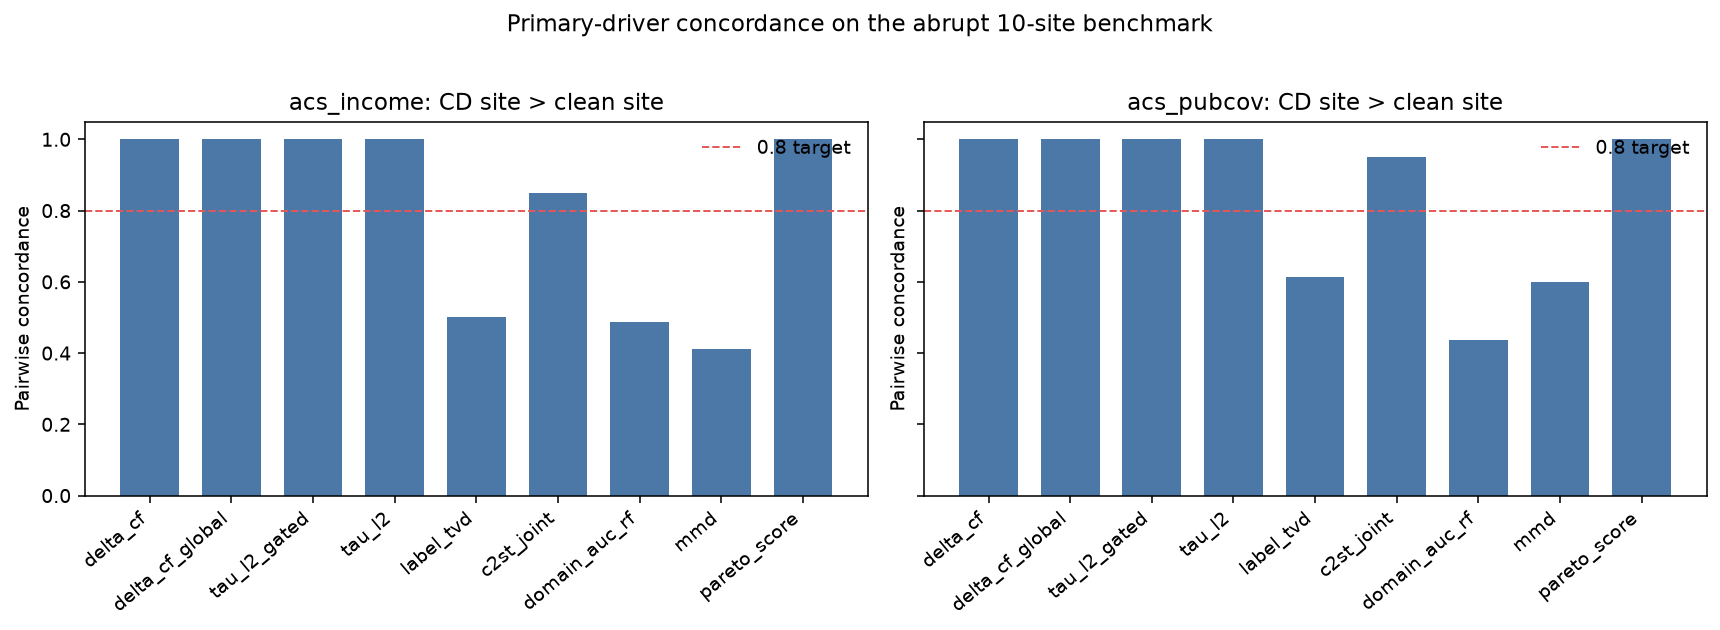
\includegraphics[width=\textwidth]{figures/concordance_cd_vs_clean.png}
\caption{主格上，各分数把概念漂移站点排在干净站点前面的比例。虚线是 \(0.8\)。来源：\texttt{concordance\_summary.csv}，四个种子。}
\label{fig:concord}
\end{figure}

\begin{figure}[ht]
\centering
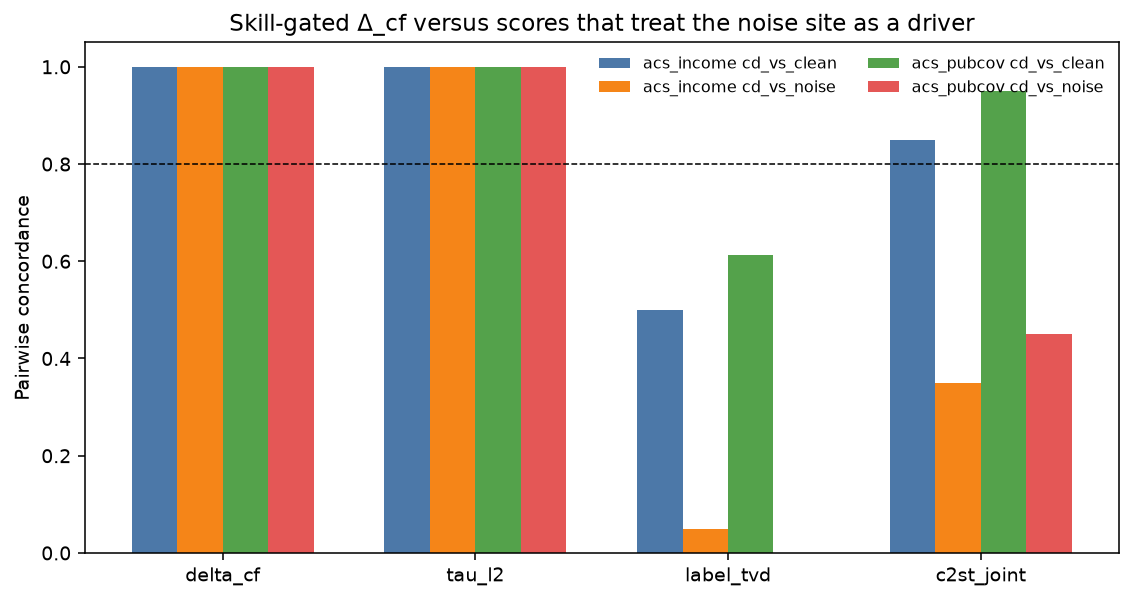
\includegraphics[width=0.92\textwidth]{figures/concordance_noise_contrast.png}
\caption{概念漂移站点相对噪声站点的一致率。合并超额、标签总变差和联合 C2ST 会把随机标签当成驱动。技能门控后的 \(\Dcf\) 保持 \(1.000\)。}
\label{fig:noise}
\end{figure}

\begin{figure}[ht]
\centering
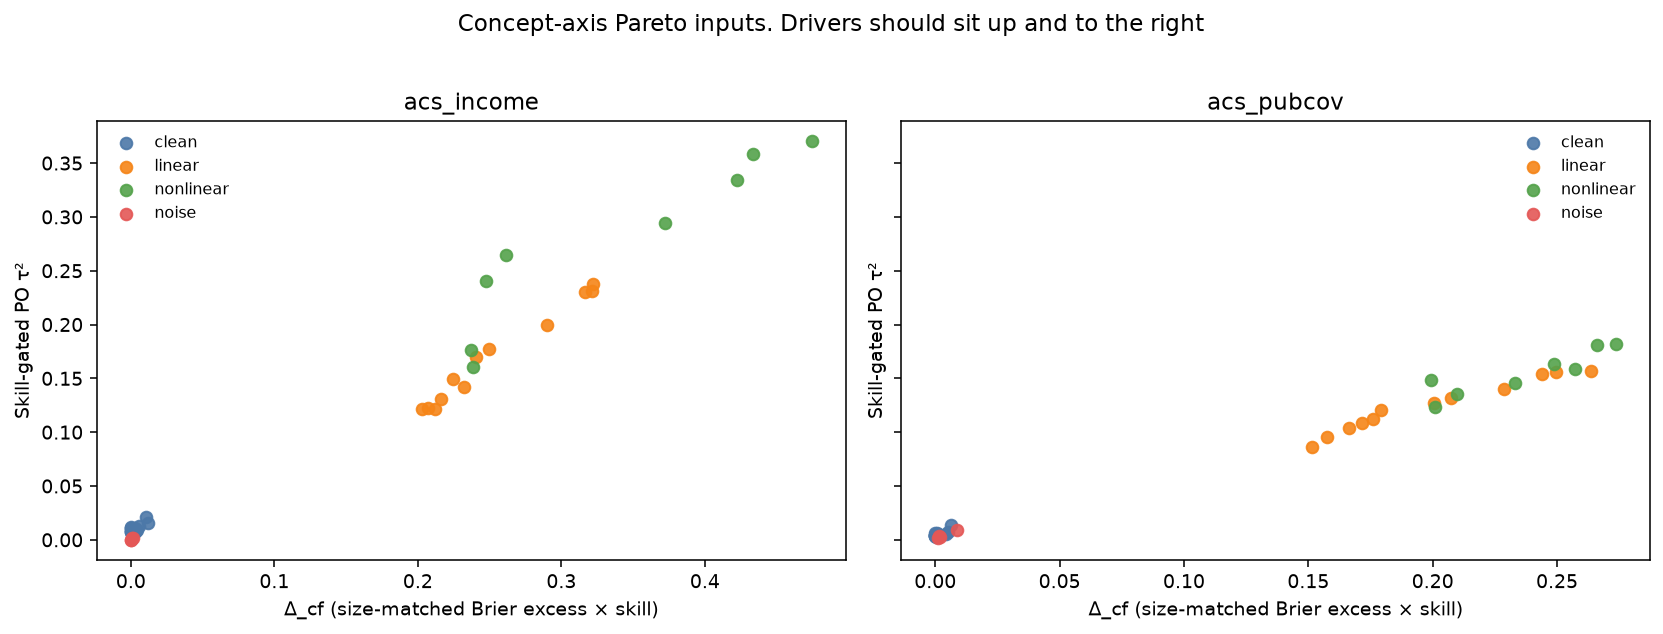
\includegraphics[width=\textwidth]{figures/pareto_inputs.png}
\caption{主格站点在 \(\Dcf\) 和技能门控 \(\tau^{2}\) 上的位置。Pareto 秩还使用了第三条轴 \(\mathrm{time\_jump}\)，图上只画了前两条。}
\label{fig:pareto}
\end{figure}

\section{漂移有没有写进去}

表\,\ref{tab:dgp} 是主格上、激活之后的标签诊断。干净站点的翻转率是 \(0\)。噪声站点的翻转率接近 \(1/2\)，激活后正例率也接近 \(1/2\)，基线正例率仍在 \(0.36\)--\(0.41\)。结构化站点的激活后正例率被拉回基线：收入线性从基线 \(0.414\) 到激活后 \(0.400\)，非线性从 \(0.420\) 到 \(0.396\)。边际标签因此不能代替概念漂移，这和表\,\ref{tab:concord-control} 里标签总变差接近 \(0.5\) 是同一件事。

\begin{table}[ht]
\centering
\caption{主格的数据生成诊断。翻转率、规则与基线的一致率、激活后正例率、基线正例率，以及线性规则实际覆盖的行比例。}
\label{tab:dgp}
\small
\begin{tabular}{@{}llrrrrr@{}}
\toprule
任务 & 类型 & 翻转率 & 与基线一致 & 激活后正例率 & 基线正例率 & 子组比例 \\
\midrule
收入 & 干净 & 0.000 & 1.000 & 0.406 & 0.406 & 0.226 \\
收入 & 线性 & 0.131 & 0.427 & 0.400 & 0.414 & 0.230 \\
收入 & 噪声 & 0.498 & 1.000 & 0.491 & 0.410 & 0.221 \\
收入 & 非线性 & 0.555 & 0.436 & 0.396 & 0.420 & 0.225 \\
医保 & 干净 & 0.000 & 1.000 & 0.369 & 0.367 & 0.494 \\
医保 & 线性 & 0.259 & 0.476 & 0.378 & 0.372 & 0.492 \\
医保 & 噪声 & 0.496 & 1.000 & 0.495 & 0.362 & 0.483 \\
医保 & 非线性 & 0.492 & 0.506 & 0.371 & 0.374 & 0.490 \\
\bottomrule
\end{tabular}
\end{table}

收入线性站点只改写大约 \(23\%\) 的行，所以翻转率 \(0.131\) 低于医保线性的 \(0.259\)。医保的 \(X_1\) 是年龄，中位数以上大约一半样本。

\section{时间}

滑动窗口长度是 \(4\)。曲线的横轴是窗口末端批次，从 \(7\) 到 \(15\)。漂移在批次 \(8\) 打开，窗口要到批次 \(11\) 才完全落进漂移，分数也在那里饱和。表\,\ref{tab:curves} 是四类站点、四个种子的 \(\Dcf\) 平均。

\begin{table}[ht]
\centering
\caption{窗口末端批次上的平均 \(\Dcf\)。\(t^{\ast}=8\)。}
\label{tab:curves}
\footnotesize
\begin{tabular}{@{}llrrrrrrrrr@{}}
\toprule
任务 & 类型 & 7 & 8 & 9 & 10 & 11 & 12 & 13 & 14 & 15 \\
\midrule
收入 & 干净 & 0.003 & 0.002 & 0.003 & 0.003 & 0.002 & 0.006 & 0.003 & 0.006 & 0.002 \\
收入 & 线性 & 0.002 & 0.005 & 0.011 & 0.070 & 0.225 & 0.223 & 0.213 & 0.231 & 0.227 \\
收入 & 非线性 & 0.002 & 0.005 & 0.022 & 0.099 & 0.330 & 0.321 & 0.309 & 0.340 & 0.310 \\
收入 & 噪声 & 0.008 & 0.004 & 0.003 & 0.003 & 0.002 & 0.005 & 0.002 & 0.004 & 0.006 \\
医保 & 干净 & 0.001 & 0.001 & 0.002 & 0.004 & 0.003 & 0.003 & 0.003 & 0.002 & 0.002 \\
医保 & 线性 & 0.002 & 0.002 & 0.015 & 0.072 & 0.184 & 0.180 & 0.189 & 0.183 & 0.185 \\
医保 & 非线性 & 0.001 & 0.002 & 0.015 & 0.060 & 0.173 & 0.178 & 0.185 & 0.173 & 0.171 \\
医保 & 噪声 & 0.003 & 0.001 & 0.001 & 0.003 & 0.006 & 0.001 & 0.004 & 0.003 & 0.002 \\
\bottomrule
\end{tabular}
\end{table}

\begin{figure}[ht]
\centering
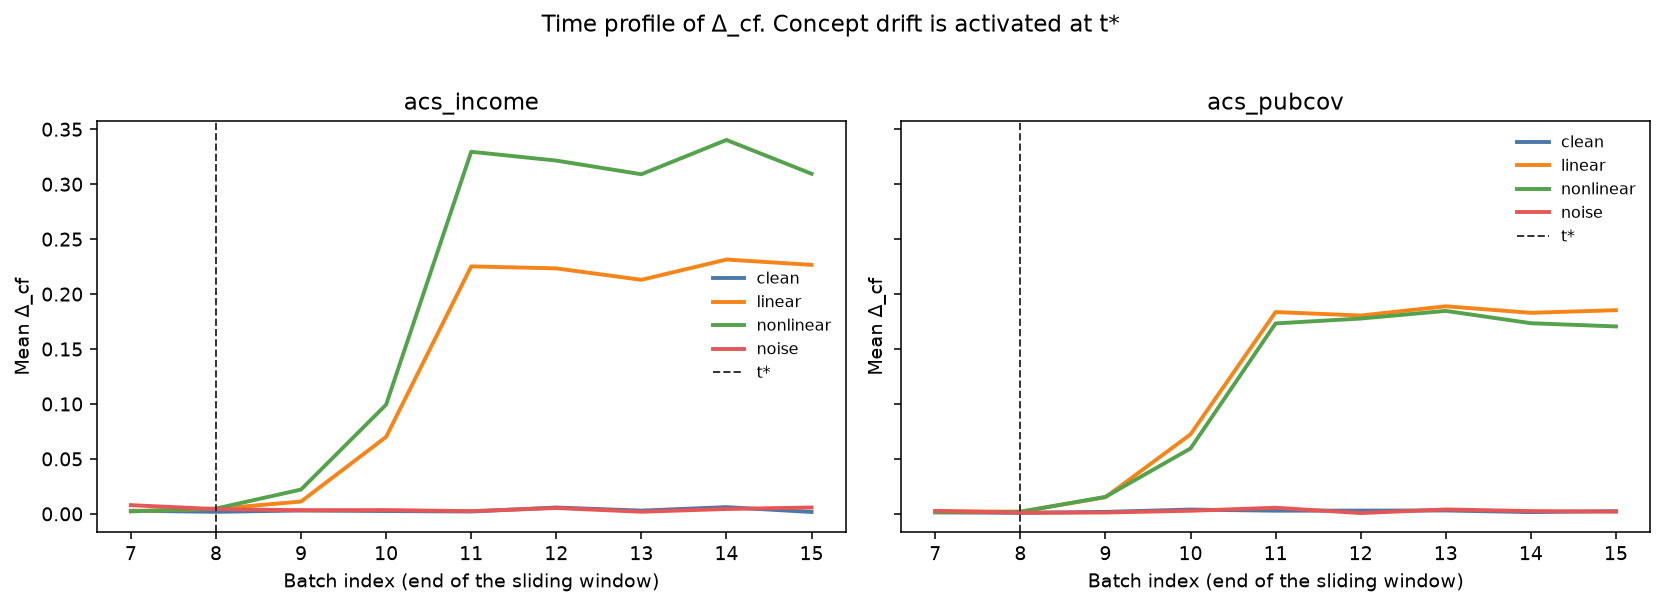
\includegraphics[width=\textwidth]{figures/time_profile_delta_cf.png}
\caption{平均 \(\Dcf\) 对窗口末端批次。竖线是 \(t^{\ast}=8\)。干净站点和噪声站点贴着零。}
\label{fig:time}
\end{figure}

在线规则用每条曲线的前两个点做校准，阈值是校准最大值加 \(0.01\)，第一次越线的窗口末端就是估计时间。命中指估计值与 \(t^{\ast}\) 相差不超过 \(2\)。在线 MAE 只在越线的站点上平均，没越线的站点（\(t_{\mathrm{online}}=-1\)）不进分母。导数时间是一阶差分最大的窗口末端，它标的是分数爬升的位置，通常比起点晚一个窗口。

误报这一列在代码里只对干净站点有定义：干净站点一旦越线就记 \(1\)。线性、非线性和噪声的误报被写成 \(0\)，不是测出来的零。表\,\ref{tab:time} 因此只对干净站点报告误报率，其余类型报告检测率。

\begin{table}[ht]
\centering
\caption{时间定位。命中率的分母是该类的全部站点。在线 MAE 的分母写在括号里，是实际越线的站点数。}
\label{tab:time}
\small
\begin{tabular}{@{}llrrrr@{}}
\toprule
任务 & 类型 & 命中率 & 干净误报 / 检测率 & 在线 MAE & 导数 MAE \\
\midrule
收入 & 干净 & 0.062 & 误报 0.375 & 4.167\,(6/16) & 4.062 \\
收入 & 线性 & 0.833 & 检测 12/12 & 1.917\,(12/12) & 2.833 \\
收入 & 噪声 & 0.250 & 检测 2/4 & 4.000\,(2/4) & 3.250 \\
收入 & 非线性 & 1.000 & 检测 8/8 & 1.625\,(8/8) & 3.000 \\
医保 & 干净 & 0.062 & 误报 0.125 & 3.000\,(2/16) & 3.875 \\
医保 & 线性 & 1.000 & 检测 12/12 & 1.417\,(12/12) & 3.000 \\
医保 & 噪声 & 0.000 & 检测 1/4 & 3.000\,(1/4) & 4.000 \\
医保 & 非线性 & 1.000 & 检测 8/8 & 1.500\,(8/8) & 3.000 \\
\bottomrule
\end{tabular}
\end{table}

非线性站点，以及医保的线性站点，命中率是 \(1\)。收入线性大约 \(0.83\)：十二个站点都越了线，有两个的越线位置超出 \(\pm 2\)。收入干净站点的在线误报率是 \(0.375\)。阈值只比校准段最大值高 \(0.01\)，短窗口上的噪声会越线，越线的位置远离 \(t^{\ast}\)，所以命中率仍然只有 \(0.062\)。

\section{类型与种植坐标}

概念组事先指定为三组充分统计量：\((X_1,X_2)\)、乘积 \(X_1 X_2\)、\((\sin X_1,\, X_3^{2})\)。组重要度是该组交叉拟合 Brier 相对截距模型的下降。类型判定取重要度最大的组。\texttt{type\_call\_all} 用最近窗口的全部行；\texttt{type\_call\_sub} 只用 \(X_1\) 高于全局分位数的子组。准确率只在五个真实漂移站点上计算，每个种子五站。Top-5 精度是按 \(\Dcf\) 取出的五个站点里真正是漂移站点的比例，八个主重复都是 \(1.000\)。

\begin{table}[ht]
\centering
\caption{五个漂移站点上的类型准确率，以及按机制合并两个任务后的召回。线性有 \(24\) 个站点--种子，两种非线性机制各有 \(8\) 个。}
\label{tab:type}
\small
\begin{tabular}{@{}llcc@{}}
\toprule
判定 & 范围 & 准确率或召回 & Top-5 精度 \\
\midrule
全样本 & 收入，五站 & 0.700 & 1.000 \\
全样本 & 医保，五站 & 0.700 & 1.000 \\
\(X_1\) 上尾 & 收入，五站 & 0.750 & 1.000 \\
\(X_1\) 上尾 & 医保，五站 & 0.900 & 1.000 \\
\midrule
全样本 & 线性半空间 & 0.500 & --- \\
全样本 & 乘积 & 1.000 & --- \\
全样本 & \(\sin(X_1)+X_3^{2}\) & 1.000 & --- \\
\(X_1\) 上尾 & 线性半空间 & 0.917 & --- \\
\(X_1\) 上尾 & 乘积 & 0.375 & --- \\
\(X_1\) 上尾 & \(\sin(X_1)+X_3^{2}\) & 1.000 & --- \\
\bottomrule
\end{tabular}
\end{table}

全样本上，乘积和正弦平方被对应的概念组认出来，线性站点只有一半。子组以外的标签仍是基线结果，加法模型会和基线结构混在一起。判定限制在 \(X_1\) 上尾之后，线性召回升到 \(0.917\)，正弦平方仍然是 \(1\)。乘积规则写在全部行上，上尾里的截断让线性拟合看起来也不差，召回降到 \(0.375\)。

种植支撑：线性和乘积是 \(\{X_1,X_2\}\)，正弦平方是 \(\{X_1,X_3\}\)。表\,\ref{tab:feature} 的 AUROC 是特征分数对这个 \(0/1\) 支撑的排序。\texttt{shift\_vimp} 是概念间隙在条件置换该坐标后的下降。\texttt{delta\_pred\_vimp} 是最近窗口的预测型置换重要度减去预烧期的同一重要度。

\begin{table}[ht]
\centering
\caption{特征支撑的 AUROC。收入每个站点 \(10\) 个特征，医保 \(19\) 个。线性 \(n=12\) 个站点--种子，非线性 \(n=8\)。}
\label{tab:feature}
\small
\begin{tabular}{@{}llrrrr@{}}
\toprule
任务 & 类型 & 预测重要度之差 & \(\ell_1\) 系数 & 预测重要度 & 概念间隙重要度 \\
\midrule
收入 & 线性 & 0.651 & 0.786 & 0.927 & 0.906 \\
收入 & 非线性 & 1.000 & 0.930 & 1.000 & 0.789 \\
医保 & 线性 & 0.944 & 0.841 & 0.995 & 0.953 \\
医保 & 非线性 & 0.985 & 0.879 & 1.000 & 0.985 \\
\bottomrule
\end{tabular}
\end{table}

\section{把十条站点收成一条支撑}

每个站点上传一条概念间隙重要度，先截断负值，再归一成单纯形。真值向量把每个漂移站点的种植坐标加一。\(\Dcf\) 加权在干净站点和噪声站点接近零时，不会把它们送进聚合。IVW 用置换重复的方差，方差下界 \(10^{-4}\)。

\begin{table}[ht]
\centering
\caption{聚合器对种植支撑的恢复。四个种子的平均。\(P@K\) 的 \(K\) 等于种植坐标的个数。}
\label{tab:agg}
\small
\begin{tabular}{@{}llrrr@{}}
\toprule
任务 & 聚合器 & AUROC & \(P@K\) & Spearman \\
\midrule
收入 & \(\Dcf\) 加权的概念间隙 & 0.917 & 0.750 & 0.697 \\
收入 & 逆方差加权 & 0.869 & 0.667 & 0.597 \\
收入 & 中位数 & 0.869 & 0.667 & 0.608 \\
收入 & 只用主驱动站点 & 0.893 & 0.667 & 0.664 \\
收入 & 均匀，预测重要度之差 & 0.869 & 0.833 & 0.600 \\
收入 & 均匀，\(\ell_1\) 系数 & 0.988 & 0.917 & 0.798 \\
收入 & 均匀，预测重要度 & 0.988 & 0.917 & 0.798 \\
收入 & 均匀，概念间隙 & 0.869 & 0.667 & 0.597 \\
收入 & 均匀，去掉噪声站点 & 0.869 & 0.667 & 0.589 \\
医保 & \(\Dcf\) 加权的概念间隙 & 1.000 & 1.000 & 0.634 \\
医保 & 逆方差加权 & 0.995 & 0.917 & 0.629 \\
医保 & 中位数 & 0.984 & 0.833 & 0.615 \\
医保 & 只用主驱动站点 & 0.995 & 0.917 & 0.630 \\
医保 & 均匀，预测重要度之差 & 0.875 & 0.833 & 0.494 \\
医保 & 均匀，\(\ell_1\) 系数 & 0.927 & 0.667 & 0.552 \\
医保 & 均匀，预测重要度 & 0.990 & 0.917 & 0.623 \\
医保 & 均匀，概念间隙 & 0.995 & 0.917 & 0.629 \\
医保 & 均匀，去掉噪声站点 & 1.000 & 1.000 & 0.635 \\
\bottomrule
\end{tabular}
\end{table}

收入上，这些种植坐标本来就会预测基线标签，所以干净站点的预测重要度也指向它们。均匀的概念间隙聚合 AUROC 是 \(0.869\)；用 \(\Dcf\) 当站点权重之后是 \(0.917\)。医保上，均匀聚合已经是 \(0.995\)，\(\Dcf\) 加权把它收到 \(1.000\)。均匀的 \(\ell_1\) 和预测重要度在收入上更高（\(0.988\)），因为它们用的是基线就能看见的预测结构，不是概念间隙。

留一站点的影响度定义为全体均匀聚合与去掉该站点之后的 Spearman 距离，\(1-\rho\)。表\,\ref{tab:loso} 里四类站点都很小，而且干净站点并不比较漂移站点更小。站点级的 \(\Dcf\) 能指出主驱动；均匀重要度聚合的留一影响度不能。

\begin{table}[ht]
\centering
\caption{留一站点影响度 \(1-\mathrm{Spearman}\)。收入干净 \(n=16\)，线性 \(n=12\)，噪声 \(n=4\)，非线性 \(n=8\)；医保同样。}
\label{tab:loso}
\small
\begin{tabular}{@{}lrrrr@{}}
\toprule
任务 & 干净 & 线性 & 噪声 & 非线性 \\
\midrule
收入 & 0.033 & 0.013 & 0.018 & 0.021 \\
医保 & 0.008 & 0.006 & 0.006 & 0.005 \\
\bottomrule
\end{tabular}
\end{table}

\FloatBarrier
\section{强度、尾部和渐进激活}

这一节只在收入任务上做。除主格外，每个格子是三个种子的轻量打分器。表\,\ref{tab:sens} 的一致率是 \(\Dcf\) 的 \(\mathrm{CD}>\mathrm{clean}\)。整窗列是同一对比下的 \(\texttt{delta\_cf\_global}\)。\(q=0.7\) 与 \(q=0.5\) 数值相同，表中省略；两列都在 CSV 里。

\begin{table}[ht]
\centering
\caption{收入任务上 \(\Dcf\) 的一致率如何随强度、激活方式和线性尾部变化。括号内是最差种子。主格一行是四个全量种子，其余是三个轻量种子。}
\label{tab:sens}
\small
\begin{tabular}{@{}rrllcc@{}}
\toprule
\(\alpha\) & \(q\) & 激活 & 平均一致率 & 最差种子 & 整窗一致率 \\
\midrule
0.4 & 0.5 & 突然 & 0.783 & 0.650 & 0.433 \\
0.4 & 0.5 & 渐进 & 0.750 & 0.650 & 0.467 \\
0.4 & 0.8 & 突然 & 0.617 & 0.450 & 0.550 \\
0.4 & 0.8 & 渐进 & 0.600 & 0.450 & 0.617 \\
0.4 & 0.9 & 突然 & 0.550 & 0.450 & 0.567 \\
0.4 & 0.9 & 渐进 & 0.550 & 0.450 & 0.567 \\
0.7 & 0.5 & 突然 & 1.000 & 1.000 & 0.933 \\
0.7 & 0.5 & 渐进 & 1.000 & 1.000 & 1.000 \\
0.7 & 0.8 & 突然 & 0.967 & 0.950 & 0.683 \\
0.7 & 0.8 & 渐进 & 0.950 & 0.900 & 0.717 \\
0.7 & 0.9 & 突然 & 0.817 & 0.750 & 0.567 \\
0.7 & 0.9 & 渐进 & 0.683 & 0.500 & 0.500 \\
1.0 & 0.5 & 突然 & 1.000 & 1.000 & 1.000 \\
1.0 & 0.5 & 渐进 & 1.000 & 1.000 & 1.000 \\
1.0 & 0.8 & 突然 & 1.000 & 1.000 & 1.000 \\
1.0 & 0.8 & 渐进 & 1.000 & 1.000 & 1.000 \\
1.0 & 0.9 & 突然 & 0.850 & 0.750 & 0.700 \\
1.0 & 0.9 & 渐进 & 0.867 & 0.800 & 0.700 \\
\bottomrule
\end{tabular}
\end{table}

\begin{figure}[ht]
\centering
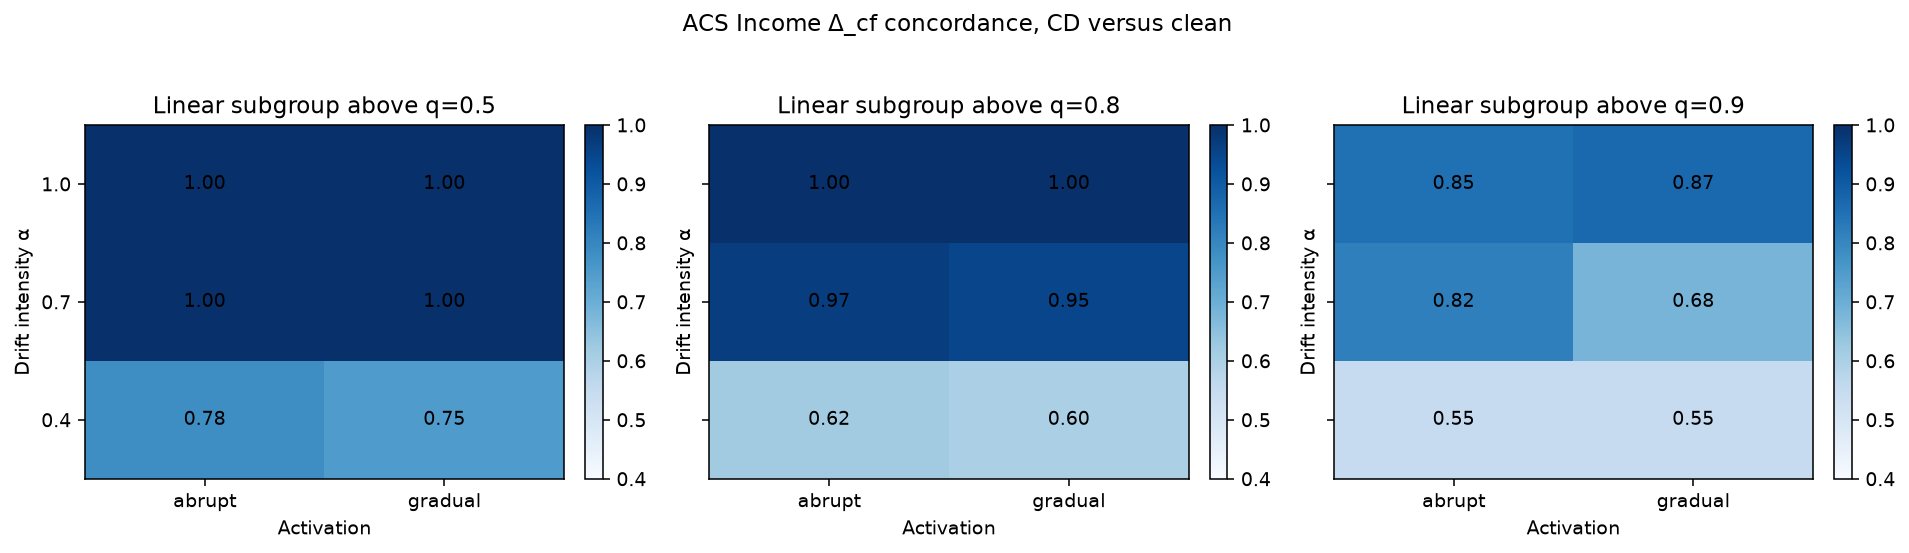
\includegraphics[width=\textwidth]{figures/sensitivity_concordance.png}
\caption{收入任务、线性子组之上，\(\Dcf\) 的 \(\mathrm{CD}>\mathrm{clean}\) 一致率。颜色是三个或四个种子的平均。\(q=0.7\) 与 \(q=0.5\) 重合，图中按分位分开画。}
\label{fig:sens}
\end{figure}

\(0.8\) 这条线在三处被踩破。\(\alpha=0.4\) 时，即使尾部仍有 \(23\%\) 的行，区域最大的一致率是 \(0.783\)（突然）和 \(0.750\)（渐进），最差种子 \(0.650\)。\(q=0.9\) 时，满强度的突然激活也只有 \(0.850\)，最差种子 \(0.750\)；\(\alpha=0.7\) 的渐进激活掉到 \(0.683\)。\(\alpha\ge 0.7\) 且尾部不少于 \(0.8\) 分位所覆盖的大约 \(17\%\) 时，平均一致率保持在 \(0.95\) 以上。

整窗分数在弱改写上更早失败。\(q=0.5\)、\(\alpha=0.4\) 时，区域最大还有 \(0.783\) / \(0.750\)，整窗只剩 \(0.433\) / \(0.467\)。仓库笔记里写的「掉到 \(0.45\) 左右」指的就是这一对，精确值是这两格。

\FloatBarrier
\section{怎么读这些数}
\label{sec:reading}

满强度、突然激活、中位数尾部这一格上，\(\Dcf\) 完成了它被要求做的排序：五个结构化漂移站点全部在四个干净站点和一个噪声站点之前，两个任务、四个种子、最差种子都是 \(1\)。Pareto 秩同样是 \(1\)。Top-5 精度是 \(1\)。

这个分离来自概念项，不来自协变量臂。随机森林 domain AUC 和 MMD 的一致率落在 \(0.4\)--\(0.6\)。逻辑回归的 domain AUC 更低，收入上 \(\mathrm{CD}>\mathrm{clean}\) 只有 \(0.300\)。站点共享 \(P(X)\)，这两条臂应当接近一半，结果也是这样。

噪声站点是另一条失败模式。收入上，合并参考 Brier 差对噪声的一致率是 \(0.400\)，标签总变差是 \(0.050\)，联合 C2ST 是 \(0.350\)。未加权 \(\tau^{2}\) 在主格上仍把噪声排在干净站点后面，是因为干净站点的 \(\tau^{2}\) 更小（\(0.015\) 对噪声的 \(0.096\) 仍小于漂移站点的 \(0.181\) 和 \(0.313\)）；技能门把噪声的 \(\tau^{2}\) 从 \(0.096\) 收到 \(0.001\)，和 \(\Dcf\) 的 \(0.001\) 对齐。等样本量 Brier 差在主格上也是 \(1.000\)。技能门在这套满强度格子里是保险，在噪声的本地 AUC 靠近 \(0.5\) 时才会改排序。收入的本地技能单独使用时，\(\mathrm{CD}>\mathrm{clean}\) 是 \(0.938\)，最差种子 \(0.800\)：非线性站点里有一把技能只有 \(0.678\) 的站点，单靠 AUC 会把它排到部分干净站点后面。

时间上，曲线的形状和窗口长度一致：批次 \(8\) 打开，批次 \(11\) 饱和。在线命中对非线性和医保线性是 \(1\)，收入线性是 \(0.833\)。收入干净站点 \(0.375\) 的越线率说明 \(0.01\) 这个门槛对短窗口偏松；越线位置的 MAE 是 \(4.17\) 个批次，离 \(t^{\ast}\) 远。导数法的误差大约一个窗口长度。

类型字典是事先指定的。全样本召回把线性站点漏掉一半；收到 \(X_1\) 上尾之后，线性召回 \(0.917\)，乘积召回 \(0.375\)。两种判定不能同时用在所有机制上。特征支撑上，预测型置换重要度和概念间隙置换重要度都能把种植坐标排到前面。留一站点的秩影响在所有类型上都很小，不能代替站点级 \(\Dcf\)。

有四件事先写明的读数限制。

\begin{enumerate}
\item 主格 Pareto 用了 \(\Dcf\)、门控 \(\tau^{2}\) 和 \(\mathrm{time\_jump}\) 三条轴。敏感性格子没有曲线，只用前两条。\texttt{RESULTS.md} 里「两条轴」只对后者成立。
\item 误报率只对干净站点有定义。其他类型在 \texttt{localize} 里被写成 \(0\)。
\item 在线 MAE 丢掉了没有越线的站点。表\,\ref{tab:time} 写了分母。
\item \(q=0.5\) 与 \(q=0.7\) 在工时上是同一次实验。敏感度表不把它们算成两次独立证据。轻量格的 C2ST 列在打分器里被填成 \(0.5\)，那些格子的 C2ST 一致率是 \(0\)，不是测量，本纪要不报。
\end{enumerate}

\FloatBarrier
\appendix

\section{同日另一份记录：条件分布反事实}
\label{app:cf}

这一节转写当天 01:53（太平洋时间）写好的画布《条件分布反事实：四张面板的五层证伪》。原始扫描不在本仓库，下面的数没有在这台检出上重算。分数是观测分布和反事实预测分布的 MMD，除以无干预基线。阈值在跑实验之前写死。画布的结论是：没有一张面板达到可以拿去决策的等级。

\begin{table}[ht]
\centering
\caption{五层判定，转自当天画布。通过线：L1 至少三种构造过线；L2 的安慰剂、峰值和门控都要过；L3 的 PIT、Wasserstein、HSIC 都要过；L4 至少三个代理同向；L5 的变异系数和 E-value 都要过。}
\label{tab:cf-layers}
\footnotesize
\begin{tabular}{@{}>{\raggedright\arraybackslash}p{3.6cm}lllllll@{}}
\toprule
面板 & MVP & L1 & L2 & L3 & L4 & L5 & 可信度 \\
\midrule
长记忆模拟，峰值在第\,10\,天 & 进入 & 通过 & 未过 & 未过 & 通过 & 未过 & 低 \\
短记忆模拟，峰值在第\,1\,天 & 进入 & 通过 & 通过 & 未过 & 通过 & 未过 & 低 \\
北京多站点 PM2.5，2014--2017 & 停止 & --- & --- & --- & --- & --- & 停止 \\
美国各州疫情，2020-03 至 2021-06 & 继续 & 假设未支持 & 未过 & 未过 & 不确定 & 未过 & 低 \\
\bottomrule
\end{tabular}
\end{table}

长记忆面板的归一化 MMD 在假设滞后 \(1\) 到 \(15\) 上是
\(0.10,\allowbreak 1.84,\allowbreak 0.22,\allowbreak 2.71,\allowbreak 4.59,\allowbreak 2.63,\allowbreak 45.5,\allowbreak 197,\allowbreak 224,\allowbreak 206,\allowbreak 0.17,\allowbreak 0.31,\allowbreak 0.39,\allowbreak 1.68,\allowbreak 10.5\)。
声明的真值是第\,10\,天（\(206\times\)），扫描最大值在第\,9\,天（\(224\times\)），差这一天，时间定位未过。第\,15\,天仍有 \(10.5\times\)，安慰剂未过。短记忆的峰值在第\,1\,天，\(2.10\times\)，其余滞后都低于 \(2\)，时间定位通过。美国南部相对东北部的十条滞后贴着 \(1\)，第\,10\,天是 \(1.00\times\)，扫描最大值在第\,1\,天（\(1.43\times\)）。

\begin{table}[ht]
\centering
\caption{模拟面板的构造、校准与敏感性，转自当天画布。}
\label{tab:cf-cal}
\small
\begin{tabular}{@{}lcc@{}}
\toprule
项目 & 长记忆 & 短记忆 \\
\midrule
剂量--反应 & 一致率 \(0.90\)，Spearman \(0.90\) & 三种构造通过；时间距离 Spearman \(-0.685\) \\
时间距离 & Spearman \(0.16\)，与峰值假设不符 & 未到 \(-0.7\)，这一组失败 \\
重叠度 & 一致率 \(0.83\)，Spearman \(0.80\) & 通过 \\
外生隔离 & 效应量 \(-2.51\)，\(p=0.034\) & 通过 \\
Wasserstein / 上限 & \(0.082\) / \(0.095\) & \(0.078\) / \(0.093\) \\
HSIC 比值 & \(0.87\) & \(0.86\) \\
PIT & 四维都拒绝均匀 & 第\,3\,维 \(p=5\times 10^{-5}\) \\
核宽变异系数（线 \(0.20\)） & \(0.71\) & \(0.25\) \\
架构变异系数（线 \(0.30\)） & \(0.23\) & \(0.00\) \\
E-value（线 \(2\)） & \(19.9\) & \(32.9\) \\
\bottomrule
\end{tabular}
\end{table}

北京，东四看古城、滞后 \(10\) 天：五段异常的排序一致率 \(0.30\)，Spearman \(-0.60\)，主查询倍数 \(0.30\)。协议在这里停止，没有训练 DDPM。美国疫情的业务窗口里南部确实异常（\(z=2.49\)），但这条 \(10\) 天的跨区反事实没有解释它；观测 PIT 和 Wasserstein 都失败，所以「没有超过基线」本身也不可信。

\end{document}
